\documentclass[a4paper,11pt,twoside, openany]{ctexbook}
% \usepackage[utf8]{inputenc}
\usepackage{ctex}
\usepackage{wallpaper} % XeLaTeX:使用wallpaper包设置封面及背景
% https://blog.yasking.org/a/xelatex-cover.html
\usepackage{amsmath}
\usepackage{bm}
\usepackage{graphicx}
% \usepackage{color}
\usepackage{tabularx}
\usepackage{hyperref}
\usepackage{float}
\usepackage{url}
\usepackage{float}   % 控制图片位置
\usepackage{geometry}
\geometry{left=2.0cm, right=2.0cm, top=2.5cm, bottom=2.5cm}
\usepackage[sectionbib]{chapterbib}  
\usepackage{cite}
% 给每章或每节加入独立的参考文献
% \usepackage{natbib}  % chapterbib会与natbib冲突
% \usepackage{biblatex}
\usepackage{tikz}

\usepackage{hyperref}
% \usepackage[colorlinks=true, linkcolor=black]{hyperref}
\hypersetup{colorlinks, citecolor=blue, filecolor=green,linkcolor=black,urlcolor=blue,
% colorlinks=false
}

\usepackage{enumerate}
\usepackage{amssymb}

\newcommand{\reffig}[1]{Figure \ref{#1}} % 需要引用图片的时候,用\reffig代替\ref

\title{医学图像文件格式大全}
\author{1595888913 }
\date{November 2018}

\begin{document}
% 封面
\begin{titlepage}
    \thispagestyle{empty}
    \noindent\fboxsep=0pt
    \ThisTileWallPaper{\paperwidth}{\paperheight}{fig/screen.png}
    \par
    \centering
    \Huge{\textbf{\textcolor{blue}{Encyclopedia of Medical Image File Formats \\ 医学图像文件格式大全}}}
    \par
\end{titlepage}
\clearpage


\maketitle
\newpage


\par
\centering
\textbf{前言}
\par


初衷:
在做图像处理与医学成像的过程中,经常与遇到各种各样的医学图像格式,包括自然图像格式jpg, png, bmp, tiff等,但更多的涉及到医学成像领域的,以及图像后处理领域的。
医学成像领域的主要包括CT, MRI, PET, US, NI, DR,X-machine等,这里涉及到不同的医学成像设备制造商,他们各自的格式也不一样。比如SIMENS的.dat格式,GE的raw格式, PHILLIP的格式,以及一些专用的医学图像格式,比如nii格式,dcm格式,mnc格式等,还有一些软件里面涉及到的格式,比如matlab里面的mat数据格式,csv格式等,对于医学图像处理软件来说,图像数据的读写和显示是首先要解决的事情,只有先解决好图像文件的读写和可视化问题,后续的重建算法,图像后处理算法方可实现。


第一章主要概述各种不同的图像格式,以及它们的相关文档,官方网站,以及相关的读写及可视化工具的介绍。


第二章详细介绍自然图像格式,比如bmp, jpg, png, tiff等格式的技术标准,以及在各种不同的编程语言环境下如何实现读写以及可视化。

第三章详细介绍医学成像过程中的各种不同的数据格式,主要从不同的成像模态来区分,同时介绍一下成像原理以及不同的数据文件格式中物理量的含义。主要涉及的医学成像模态主要包括MRI,CT,DR, PET, US, NI, SPECT等。其中MRI数据是k空间数据,CT数据是正弦图sinograms数据, PET是






\tableofcontents

\listoftables 

\listoffigures


\chapter{医学图像概文件格式概述}


\begin{figure}[H]
    \centering
    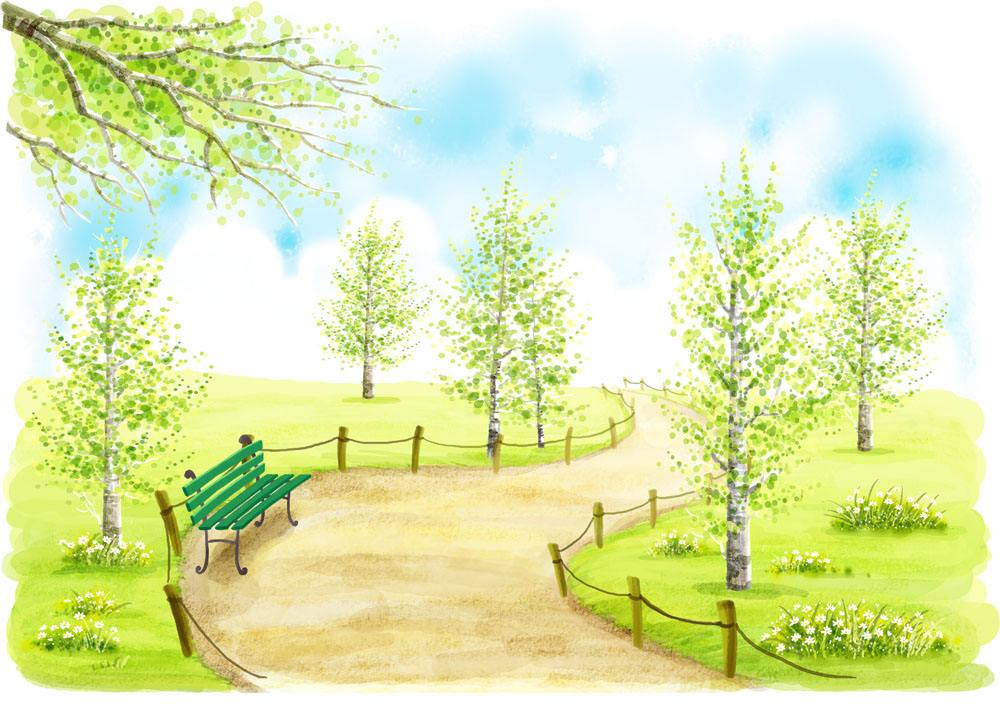
\includegraphics[width=8cm, height=8cm]{fig/screen.png}
    \caption{封面图}
    \label{fig:1-1}
\end{figure}
\section{常见的医学图像格式}
\section{医学图像格式的读写与可视化}
\section{不同类型的文件格式官网及技术标准}
\section{小结}


\chapter{自然图像格式的读写与可视化}
\section{自然图像格式概述}
自然图像格式主要包括bmp, jpg, png, tif等
\begin{table}[H]
    \centering
    \begin{tabular}{c|c|c|c}
        \hline 
         自然图像格式 & 官网 & 技术标准 & 备注  \\
        \hline
         bmp & & & \\ 
         jpg & & & \\ 
         pnp & & & \\ 
         tif & & & \\ 
        \hline
    \end{tabular}
    \caption{自然图像格式汇总表}
    \label{tab:2-1}
\end{table}


\section{常见的自然图像格式}
\subsection{bmp}
\subsection{jpg}
\subsection{png}
\subsection{tif}
\section{小结}




\chapter{医学图像格式的读写与可视化}
\section{医学图像格式概述}
\section
常见的医学图像包括dcm, nii, mnc, cfi, raw, dat等
\begin{table}[H]
    \centering
    \begin{tabular}{c|c|c|c}
        \hline 
         医学图像格式 & 官网 & 技术标准 & 备注  \\
        \hline
         dcm & & & \\ 
         nii & & & \\ 
         mnc & & & \\ 
         raw + hdr & & & \\ 
         raw + hdr & & & \\ 
        \hline
    \end{tabular}
    \caption{医学图像格式汇总表}
    \label{tab:3-1}
\end{table}

\subsection{dcm}
\subsubsection{格式技术标准}
\subsubsection{官网及资料}
\subsubsection{相关读写与可视化工具}
\subsection{nii}
\subsection{mnc}
\subsection{raw}
\section{小结}
\input{chp/chp4.tex}
\input{chp/chp5.tex}
\input{chp/chp6.tex}
\input{chp/chp7.tex}
\input{chp/chp8.tex}
\input{chp/chp9.tex}
\input{chp/chp10.tex}
\input{chp/chp11.tex}
\input{chp/chp12.tex}
\input{chp/chp13.tex}
\input{chp/chp14.tex}
\input{chp/chp15.tex}
\input{chp/chp16.tex}
\input{chp/chp17.tex}
\input{chp/chp18.tex}
\input{chp/chp19.tex}
\input{chp/chp20.tex}
\end{document}
